\section{Results}
\subsection{Quantitative results}

We will discuss our quantitative results in terms of the three
measures that we have proposed earlier in the paper.

\subsubsection{Keystrokes Per Character (KSPC)}

KSPC is generally treated as a measure of accuracy, because it
represents the number of keystrokes executed per character. From our
experiment, it turned out that all the three mechanisms were similar
in terms of KSPC measurements as shown in
Table~\ref{tab:KSPCStatisticsForTextCorpora}.

\begin{table*}
\begin{minipage}[b]{0.5\linewidth}
	\centering
		\begin{tabular}{|l|c|c|c|} \hline
		                         & Avg. KSPC & Max. KSPC & Min. KSPC \\ \hline
			 QWERTY & 1.288 & 1.325 & 1.239 \\ \hline
			 Chording & 1.261 & 1.373 & 1.110 \\ \hline
			 Bksd. QWERTY & 1.338 & 1.497 & 1.278 \\ \hline
		\end{tabular}
	\caption{KSPC Statistics}
	\label{tab:KSPCStatisticsForTextCorpora}
\end{minipage}	
\begin{minipage}[b]{0.5\linewidth}
	\centering
		\begin{tabular}{|l|c|c|c|} \hline
		                         & Avg. WPM & Max. WPM & Min. WPM \\ \hline
			 QWERTY & 12.162 & 15.233 & 10.2 \\ \hline
			 Chording & 4.061 & 4.79 & 2.722 \\ \hline
			 Bksd. QWERTY & 8.598 & 10.055 & 5.432 \\ \hline
		\end{tabular}
	\caption{WPM Statistics}
	\label{tab:WPMStatisticsForTextCorpora}
\end{minipage}
\end{table*}

The Chording mechanism was on an average faster than the other two
mechanisms, with the Backside QWERTY being the slowest in terms of
average. However, when we did a t-test between KSPC measurements for
QWERTY and chording mechanism, the p-value turned out to be 0.35. This
suggests that over the test subjects there was no significant
difference between the accuracies of the QWERTY and the chording
mechanisms. Similarly, a t-test between KSPC measurements for QWERTY
and backside QWERTY resulted in a p-value of 0.24, which still lacks
significance. Therefore, both the backside touch input mechanisms were
as accurate as the QWERTY mechanism.

\subsubsection{Words Per Minute (WPM)}

Words Per Minute (WPM) is a measure that is commonly used to represent
the speed of a text input mechanism. Our experiment findings suggested
that QWERTY was still the fastest mechanism, followed by backside
QWERTY and the slowest was chording. Statistics on WPM measurements
can be found in Table 3.  The results suggested that QWERTY was faster
than both backside QWERTY and chording mechanisms. However, it should
be noted that the test sessions were generally around 20-30 minutes,
and each user only interacted with a mechanism once. Therefore, the
fact that backside QWERTY was on a average 3/4th as fast as the QWERTY
mechanism was encouraging. This led us to explore the results
qualitatively and also in terms of speed versus accuracy trade-off.

\subsubsection{Speed versus Accuracy Trade-off}

In spite of the discussions above, we should acknowledge that none of
these measures can be studied totally independently, and there was a
possibility that the participants were being more accurate by
sacrificing on speed. However, since speed with a particular input
mechanism is often attributed to the amount of exposure and practice,
we had reasons to believe that the comparison of accuracies was still
fair. However, we still did some Speed vs Accuracy analysis for the
three mechanisms and [Figure] is a plot of the same.

\subsubsection{Sample tests}

Since the amount of exposure that the users received during the
sessions was limited, it was obvious that lack of experience with the
mechanisms is also hampering the speed and accuracy
measurements. Therefore, one of the researchers who was involved in
development of the interface and had reasonable exposure to the
interface went through the test in exactly the same fashion as the
participants. This was done to test the capability of the two new
mechanisms in terms of speed and
accuracy. Table~\ref{tab:StatisticsForTestCorpora} shows the
measurements from the same.

\begin{table*}
	\centering
		\begin{tabular}{|l|c|c|c|} \hline
		                         & WPM & KSPC \\ \hline
			 Chording & 7.69 & 1.12 \\ \hline
			 Backside QWERTY & 13.231 & 1.152 \\ \hline
		\end{tabular}
	\caption{Sample Measurements}
	\label{tab:StatisticsForTestCorpora}
\end{table*}

It can be seen from the table that with decent amount of exposure to
the interface, both the accuracy and the speed seem to show better
trends. However, these measurements are restricted to an individual
and are highly preliminary. To fully establish our claims, larger and
longer studies would have to be conducted.

\subsection{Qualitative results}

As mentioned earlier, the NASA task load index was used to get
subjective ratings on qualitative aspects of the interfaces. This was
just done for the two new mechanisms that were implemented. This was
done deliberately because the participants were asked to give the
ratings keeping in mind their experience with soft-QWERTY
keyboards. Since all the participants in the study had prior exposure
to soft-QWERTY keyboards, this factor was uniform through the
experiment. In the following few paragraphs we summarize the
high-level trends that were derived from the ratings that the
participants assigned to the backside QWERTY and chording
mechanisms. Figure~\ref{fig:tlx-ratings} presents the ratings given by
the users of all three mechanisms.

\subsubsection{Mental Demand}

By just looking at the ratings on the mental demand of the task on the
NASA-TLX scale, it seemed that the users reported less mental load for
the backside-QWERTY as compared to the chording mechanism. When we
conducted a t-test on the ratings, it turned out to have a p-value of
0.02, which suggests that the difference was significant. It also
means that the backside-QWERTY has significantly less mental load than
the chording mechanism. However, the average for backside-QWERTY was
29.5 and that for chording was 43, which means that on an absolute
scale participants thought that the two mechanisms were not mentally
intensive to work with. The chording mechanism was deemed as harder to
understand because in that case, the users were trying to work with
the number of fingers as a method of input. This setup was new for all
the participants in the study, and this also relates back to the low
speed (in WPM) of text entry on the chording mechanism. The averages
are lower than 50 for both the mechanisms, which denotes that quite a
few participants believed that the mechanisms are simpler to
understand and use than QWERTY. This effect was more well defined for
backside-QWERTY (average of 29.5), as opposed to chording (average of
43).

\subsubsection{Physical Demand}

An analysis of the physical demand ratings on the NASA-TLX suggested
that the participants in general found the chording mechanism to be as
physically challenging than the backside-QWERTY. Looking at the kernel
density plots of the two revealed that the distribution of population
across ratings was very similar in the two interfaces. Also a t-test
on the two sets of ratings resulted in a value of 0.91, which meant
that the difference was not significant. Therefore, it is reasonably
fair to say that the two mechanisms were equally easy or equally hard
to use. However, since the averages of both the sets of ratings were
around 50 (10 on the original scale) it means that none of the
mechanisms were exceptionally hard to use, as opposed to each
other. This also means that the two mechanisms were on an average as
easy to use as the QWERTY mechanism, since the participants were
assuming the QWERTY mechanism to have a rating of 10 (on the 20 point
scale) for all metrics.

\subsubsection{Temporal Demand}

This metric was important in the sense that we wanted to make sure
that the participants do not feel rushed during the task. Our aim was
to reproduce the natural experience of entering text, as far as
possible. Therefore, the low average scores (27.5 for both mechanisms)
suggested that the task was not pushing the participants to an extent
that they start noticing it. There were constraints that we had
specified, but none of them seemed to upset the participants. The fact
that there was no time limit to the task, was helpful in this respect.

\subsubsection{Performance}

The NASA-TLX index ratings for performance suggested that both the
interfaces had good performance. The average performance ratings for
both the interfaces were below 8 (on 20 point scale). It should be
noted that a low rating on this scale means good performance. We also
observed that there were two users who gave the chording mechanism a
higher rating, thereby implying that it did not have good
performance. Both these participants had writing speeds that were lass
than the average. This suggests that these participants were
struggling to get accustomed to the device and the mechanism. Their
speed was suffering as a result of the same. We also looked at the
videos from those sessions, and they corroborated the same claim.

\subsubsection{Effort}

The difference between the sets of ratings for backside-QWERTY and
chording was not significant. The t-test results in a p-value of
0.52. However, studying the kernel density plots (see
Figure~\ref{fig:tlx-ratings} more carefully suggested that the
distribution of the opinion on the amount of effort involved in
working with the backside-QWERTY was bimodal. However, for the
chording it was almost evenly distributed around the average
rating. The videos suggested that some of such cases were because the
backside-QWERTY did not allow for change in size of the keyboard,
people who had fingers longer or shorter than average finger sizes had
a harder time with the mechanism as opposed to other. The chording
mechanism on the other hand, did allow for such changes and therefore
got an even distribution of ratings.

\begin{figure*}
    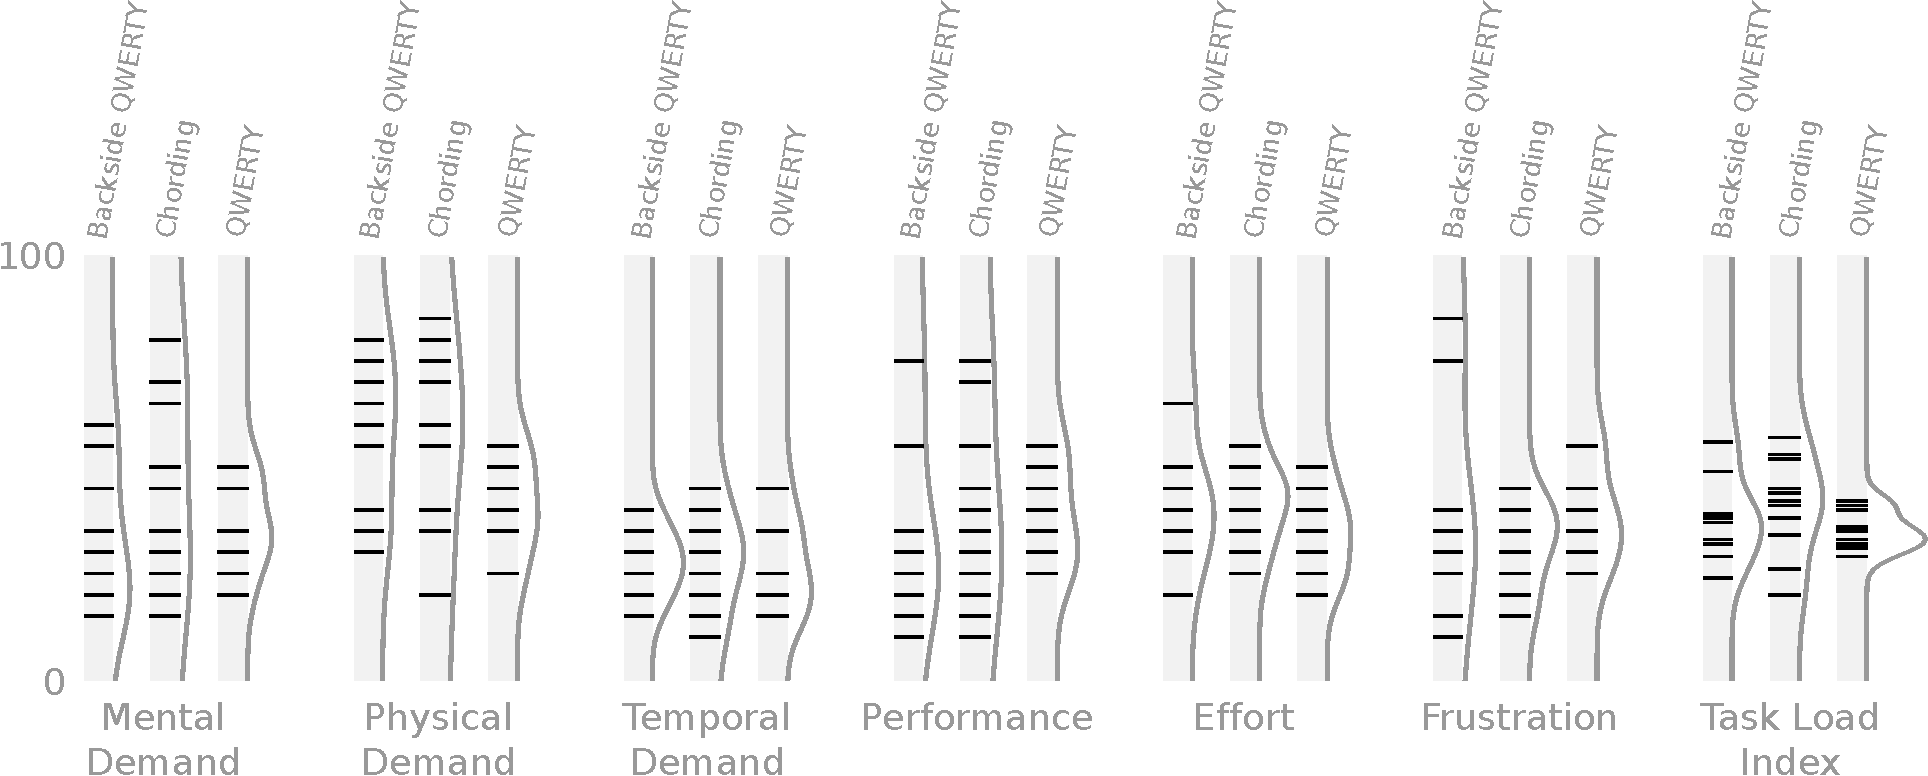
\includegraphics[width=\textwidth]{Figures/hash_and_densities_index.pdf} 
    \caption{NASA-TLX rating for all three input mechanisms}
    \label{fig:tlx-ratings}
\end{figure*}


\subsubsection{Frustration}

The ratings suggested that on an average users were satisfied with the
mechanisms. The frustration levels/ratings were restricted to the
lower half of the scale for chording, however only two users reported
higher levels of frustration with the backside-QWERTY. When we
cross-checked this with our video logs, it turned out that both of
these users had issues with getting accustomed to the mechanisms
primarily because of finger sizes, as pointed out in the last
section. This in turn resulted in the observed frustration on the
NASA-TLX.

\subsubsection{Mean Weighted Scores}
After the individual analysis of the ratings, we used the standardized
methods to calculate the effective weighted task load ratings, as
specified by NASA. Right after filling up the survey, the participants
were also asked to compare metrics against each other. Since there
were 6 metrics (Mental, Physical, Temporal, Performance, Effort,
Frustration), there were $C_{2}^{6}$ possible combinations, and 15
questions in total. After receiving all the responses from the
participants, we found that on an average effective weights for Mental
Demand, Physical Demand, Temporal Demand, Performance, Effort,
Frustration were 4, 3, 3, 1, 2, 2 respectively. In simple words, a
higher weight means that particular dimension or metric has larger
effect towards the load of the task and should be given more weightage
as opposed to others. Initially we thought that interactions with
backside-QWERTY and chording mechanisms were intrinsically different
tasks, and therefore the weights should not be treated as the
same. However, the average weights that were calculated for the two
mechanisms turned out to be very close to each other. This is
understandable from a viewpoint that both the tasks were actually text
entry tasks with same corpus, and same kind of input
method. Therefore, the value that the participants were attaching to
each metric didn't change.

It is apparent from the discussion above, but to clarify again, a low
weighted score on the NASA-TLX means that the overall task load was
low and the experience was pleasant. The backside-QWERTY obtained a
weighted score of 37 on an average, and the chording mechanism got an
average score of 41. The t-test between the two resulted in a p-value
value of 0.22, which means that the difference between the two sets of
effective ratings was not significant. The weighted scores for both
the mechanisms were low, and since the participants were comparing the
mechanisms with their experiences with soft-QWERTY, it can be seen
that the two new mechanisms were definitely welcome by the
participants. From a qualitative standpoint, the mechanisms seemed to
create good user experience, even better than a soft-QWERTY in some
cases.

\subsection{Design guidelines}

After a qualitative and quantitative analysis of our results, we also
did a high-level analysis of our design choices and cross-checked them
against the videos. As a result of this, we came up with some major
design takeaways from this piece of research. Therefore, in this
section we propose some design guidelines for future efforts that look
into text input by utilizing a backside touch input device. These
guidelines are not sufficient, but should definitely be treated as
necessary.

\subsubsection{Movement minimization}

During the study we realized that the amount of movement involved in
selecting a particular character determines the speed that users would
achieve with the mechanism. The post-experiment analysis of usability
test videos corroborated this claim. Once we reduced the size of the
keys and magnified the movement of fingers, the users could cover
larger distances with smaller shifts in position. We also realized
that users are able to control the finger position with very high
accuracy, and therefore these optimizations help them enter text at
higher speeds.

\subsubsection{Multiple finger sizes}

There can be a lot of variation in finger sizes, amongst users. We
accounted for this in the chording mechanism, by having settings that
user could select, if they had fingers larger or shorter than the
average. This was critical for chording mechanism as the users were
trying to form chords at specific locations. For backside-QWERTY, we
did not make this optimization because users were not trying to
position multiple fingers at the same time, and also because in that
case we had tried to optimize between finger movement and key
sizes. Dynamically determining the trade-off between the two,
depending on the finger size would have interfered with the optimal
setting of the system, and influenced other factors.

\subsubsection{Reducing dimensions of movement}

This one is only true for the chording mechanism, but it turned out
from the experiment that a good way to maximize on accuracy is to
reduce the number of dimensions of movement. Traditionally, with a
soft-QWERTY users tend to position themselves in both, x and y
co-ordinate. In the chording mechanism, the y direction was being
controlled by the number of fingers, and therefore the movement was
just restricted to the x direction.

\subsubsection{Visual search vs Recall}

After the usability testing, we also realized that users tend to do a
visual search to find characters instead of recalling from their
previous experiences with QWERTY mechanisms. It turned out the the
layour of keys should be visually intuitive and familiar. As long as
the positions of characters follow a pattern, either pre-existing
(like QWERTY) or familiar (alphabetic), users will be able to accustom
themselves in a few interactions.

\subsubsection{Pressure vs Touch}

As explained earlier, we also experimented with using pressure as a
mode of input, but it turned out that it is hard for users to
accurately control the amount of pressure being applied. This results
in high error rates because of spurious inputs. A design fix that we
used to mitigate the situation was to use touch on the front
screen. Since the two thumbs are anyway used to hold the device, it
was easy for the users to use them to tap on the front screen. This
significantly reduced error rates from the test version to the final
version.

\subsubsection{Touch Cursors}

Both our mechanisms involved showing finger positions on the screen,
and we had to this in a way that we don't hide any information or
don't cause a loss of perception. We achieved this by doing a number
of things. We made the touch cursors transluscent, so that we don't
occlude any information. We also kept the size of the cursor smaller
than the size of an individual key so that they are easier to position
and don't end up selecting multiple keys at the same time.
